\chapter{Implementation of Monsoon Crop Price Estimation System}

The implementation of the monsoon crop price estimation system represents a comprehensive integration of machine learning algorithms, modern web technologies, and robust data management practices specifically designed to assist farmers in making informed decisions about soybean and onion crop pricing. This chapter presents the detailed technical implementation encompassing the development of predictive models using Python-based machine learning frameworks, the creation of a responsive web application utilizing React and Node.js technologies, and the establishment of a scalable database architecture for efficient data storage and retrieval. The implementation follows a full-stack approach that bridges the gap between complex predictive analytics and user-friendly interfaces, ensuring that farmers can easily access and interpret crop price forecasts. The system architecture emphasizes modularity, scalability, and real-time data processing capabilities to provide accurate monsoon season price predictions for agricultural stakeholders.

\section{Contents of this chapter}

This chapter should elaborate the following in detail.

\begin{enumerate}
\item Machine Learning Model Implementation and Training Pipeline
\item Backend System Architecture and API Development
\item Frontend User Interface Design and Implementation
\item Database Design and Data Management System
\item Integration and System Testing Procedures
\end{enumerate}

\vspace{0.75cm}

\section{System Architecture Overview}

The monsoon crop price estimation system follows a multi-layered architecture comprising external data sources, presentation layer, application layer, machine learning layer, and data layer, as illustrated in Figure~\ref{fig:system_architecture}. The system architecture integrates machine learning capabilities with modern web technologies to deliver real-time price predictions for soybean and onion crops during monsoon seasons.

\begin{figure}[h]
\centering
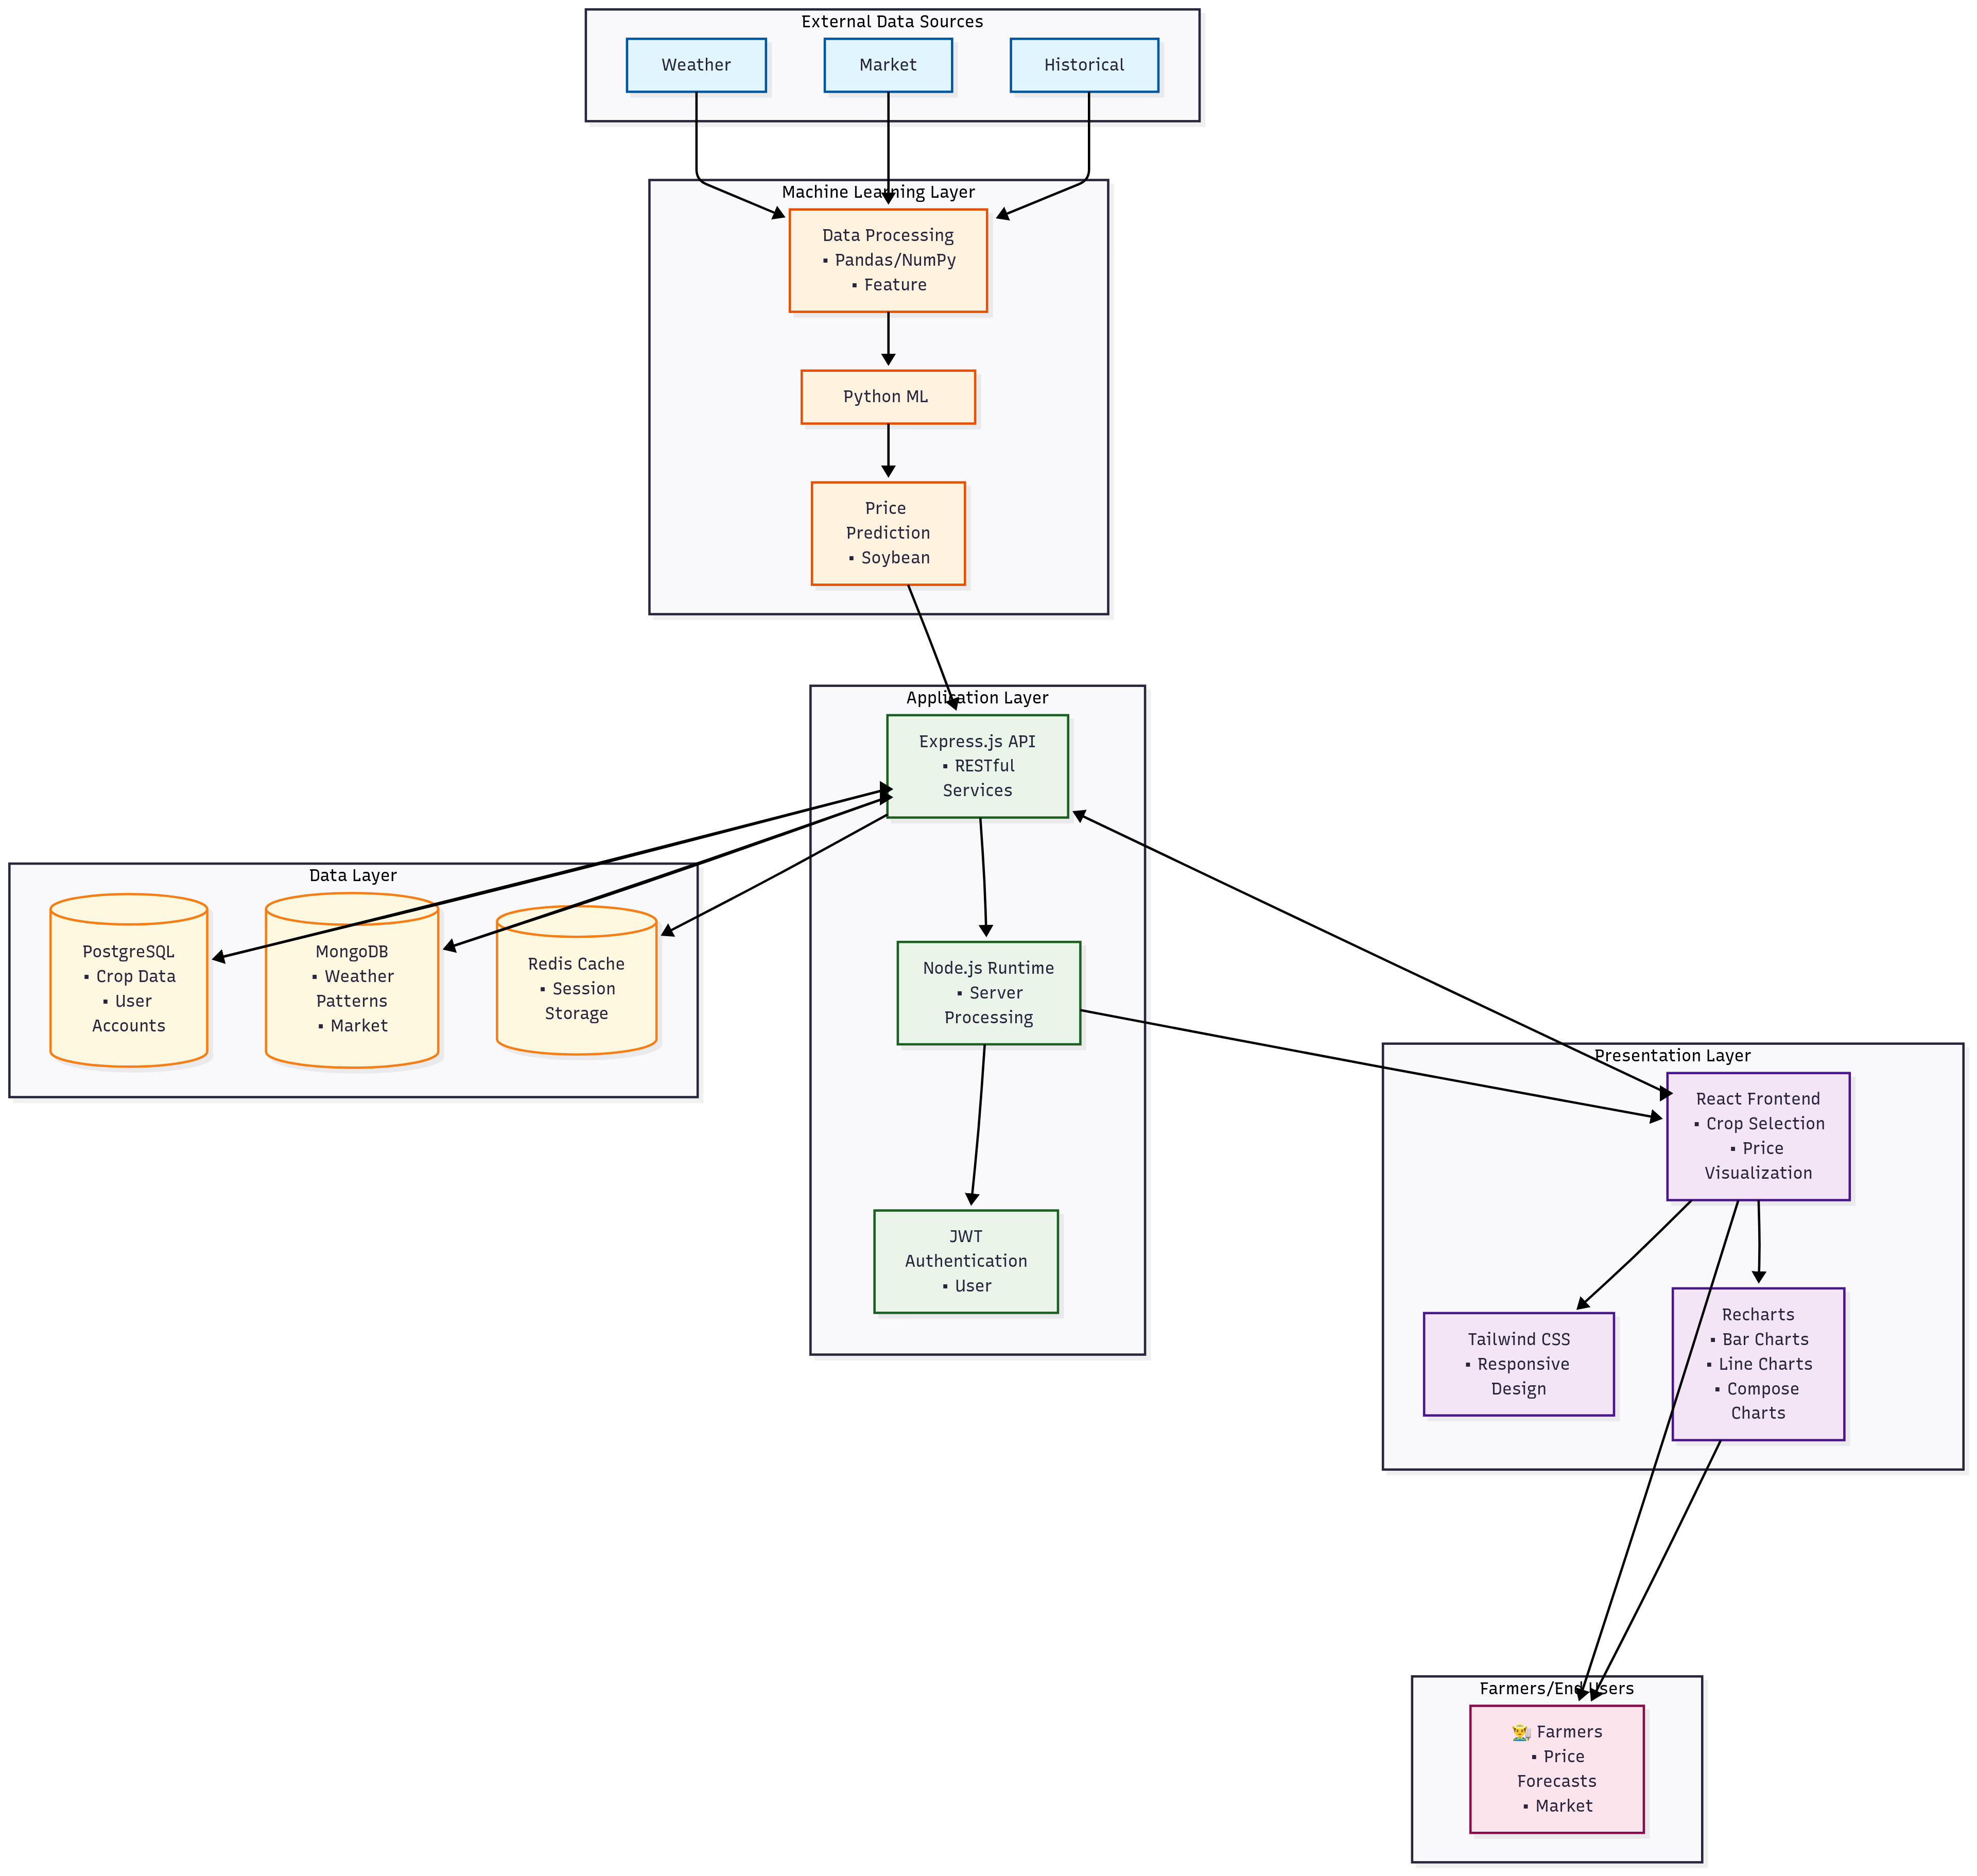
\includegraphics[width=\textwidth]{Chapter4/system_architecture.png}
\caption{System Architecture Overview for Monsoon Crop Price Estimation}
\label{fig:system_architecture}
\end{figure}

The top-level design demonstrates the flow of data from external sources through the machine learning pipeline to the user interface. The presentation layer handles user interactions and data visualization using React and Tailwind CSS, while the application layer manages business logic and RESTful API services through Node.js and Express. The machine learning layer processes agricultural data using Python-based algorithms to generate price predictions, and the data layer ensures efficient storage and retrieval through PostgreSQL, MongoDB, and Redis caching. The system seamlessly integrates weather data, market information, and historical price patterns to provide farmers with accurate crop price forecasts during monsoon seasons.

\section{Machine Learning Model Implementation}

\subsection{Model Architecture and Framework Selection}

The core predictive component of the system leverages Python-based machine learning frameworks to build robust price estimation models for soybean and onion crops during monsoon seasons. The implementation utilizes scikit-learn as the primary machine learning library, complemented by pandas for data manipulation and numpy for numerical computations. The model architecture incorporates multiple regression techniques including Random Forest, Support Vector Regression, and Gradient Boosting algorithms to ensure accurate price predictions across varying market conditions.

The training pipeline implements a comprehensive data preprocessing workflow that handles missing values, outlier detection, and feature engineering specific to agricultural price patterns. Feature selection algorithms identify the most significant variables affecting crop prices, including historical price trends, weather patterns, market demand indicators, and seasonal variations. The implementation includes automated hyperparameter tuning using GridSearchCV and cross-validation techniques to optimize model performance and prevent overfitting.

\subsection{Data Processing and Feature Engineering}

The system implements sophisticated data preprocessing techniques to transform raw agricultural and market data into meaningful features for price prediction. The preprocessing pipeline includes data normalization, categorical encoding, and temporal feature extraction to capture seasonal patterns and market cycles. Weather data integration incorporates rainfall patterns, temperature variations, and humidity levels specific to monsoon seasons, which significantly impact crop yields and subsequent pricing.

Feature engineering processes create derived variables such as price volatility indices, moving averages, and seasonal trend indicators that enhance the model's predictive accuracy. The implementation includes automated data quality checks and validation procedures to ensure data integrity throughout the processing pipeline. Real-time data ingestion capabilities allow the system to incorporate the latest market information and weather updates for dynamic price predictions.

\section{Backend System Architecture}

\subsection{RESTful API Development with Node.js and Express}

The backend infrastructure utilizes Node.js runtime environment with Express.js framework to create a scalable and efficient server-side architecture. The RESTful API design follows industry best practices with clear endpoint definitions for crop data management, price retrieval, and user authentication. The implementation includes comprehensive CRUD operations for managing crop entries, historical price data, and user preferences through well-structured HTTP endpoints.

The API architecture incorporates middleware components for request validation, error handling, and security measures including CORS configuration and Helmet.js for HTTP header security. JWT (JSON Web Tokens) authentication ensures secure access to protected resources, while bcrypt provides robust password hashing for user account security. The backend implements efficient data aggregation logic for seasonal filtering and price trend analysis, optimizing database queries for improved response times.

\subsection{Database Integration and ORM Implementation}

The system utilizes a hybrid database approach combining PostgreSQL for structured data storage with MongoDB for flexible document-based requirements. The PostgreSQL database stores critical relational data including crop information, historical prices, and user accounts, while MongoDB handles unstructured data such as weather patterns and market analysis reports. Sequelize ORM facilitates seamless interaction with PostgreSQL, providing model definitions, migrations, and query optimization features.

The database schema design incorporates proper indexing strategies for efficient data retrieval, foreign key relationships for data integrity, and stored procedures for complex analytical queries. The implementation includes automated backup procedures and data replication mechanisms to ensure system reliability and data availability. Connection pooling and query optimization techniques minimize database load and improve overall system performance.

\section{Frontend User Interface Implementation}

\subsection{React Component Architecture}

The frontend implementation leverages React's component-based architecture to create a modular and maintainable user interface specifically designed for agricultural stakeholders. The component hierarchy includes specialized components for crop selection, price visualization, seasonal filtering, and user dashboard functionality. The implementation follows React best practices including proper state management, component lifecycle optimization, and efficient rendering techniques.

The system implements conditional rendering mechanisms that adapt the interface based on seasonal variations and user preferences. React Router provides seamless navigation between different application sections, while Axios handles HTTP requests for API communication. The component design emphasizes reusability and scalability, allowing for easy extension to support additional crops and market features.

\subsection{Responsive Design with Tailwind CSS}

The user interface implementation utilizes Tailwind CSS utility-first approach to create responsive and visually appealing designs that work across various devices and screen sizes. The styling implementation includes custom color schemes, typography selections, and spacing configurations optimized for agricultural data presentation. The responsive design ensures optimal user experience on both desktop and mobile devices, accommodating farmers who may access the system from various locations.

The implementation includes interactive elements such as dropdown menus for crop selection, date pickers for seasonal filtering, and hover effects for enhanced user engagement. Tailwind's utility classes enable rapid prototyping and consistent styling across all application components, while custom CSS extensions handle specific agricultural data visualization requirements.

\section{Data Visualization and Analysis}

\subsection{Chart Implementation with Recharts}

The system incorporates comprehensive data visualization capabilities using Recharts library to present crop price trends and market analysis in intuitive graphical formats. The implementation includes bar charts for displaying price comparisons across seasons, line charts for trend analysis, and pie charts for crop distribution visualization. The visualization components support dynamic data updates and interactive features such as tooltips, zoom functionality, and data filtering options.

The chart implementations include specialized visualizations for agricultural data including seasonal price patterns, regional variation heatmaps, and forecast accuracy indicators. The system supports multiple chart types and customization options, allowing users to select preferred visualization formats based on their analytical needs. Real-time data binding ensures that visualizations automatically update when new price data becomes available.

\subsection{Advanced Analytics and Filtering}

The frontend implementation includes sophisticated filtering mechanisms that enable users to analyze price data based on specific criteria such as crop type, geographical region, and time periods. The filtering system supports multiple selection options and dynamic query generation for customized data analysis. Advanced features include price trend calculations, volatility analysis, and comparative studies between different crops and seasons.

The implementation incorporates predictive analytics visualizations that display forecast confidence intervals, model accuracy metrics, and scenario analysis results. Interactive dashboard components allow users to explore different market scenarios and understand the factors influencing price predictions. The system provides export functionality for sharing analysis results and generating reports for agricultural planning purposes.

\section{System Integration and Testing}

\subsection{API Integration and Data Flow}

The complete system integration involves seamless communication between the machine learning models, backend APIs, and frontend components through well-defined data flow protocols. The integration architecture ensures that price predictions from the ML models are efficiently processed by the backend and delivered to the frontend in real-time. The implementation includes error handling mechanisms, retry logic, and fallback procedures to maintain system stability under various operational conditions.

The data flow implementation incorporates caching strategies to optimize performance and reduce computational overhead. Redis cache integration stores frequently accessed price data and model predictions, while background job processing handles intensive computational tasks without affecting user experience. The system includes monitoring and logging capabilities to track performance metrics and identify potential bottlenecks.

\subsection{Testing Framework and Quality Assurance}

The implementation includes comprehensive testing procedures covering unit tests, integration tests, and end-to-end testing scenarios specific to agricultural price prediction requirements. The testing framework validates model accuracy, API functionality, and user interface responsiveness across different usage scenarios. Automated testing pipelines ensure code quality and system reliability through continuous integration practices.

The quality assurance process includes performance testing to validate system scalability under high user loads, security testing to verify data protection measures, and usability testing with actual farmers to ensure interface effectiveness. The testing implementation covers edge cases such as extreme weather conditions, market volatility, and data availability issues that commonly affect agricultural price predictions.

\vspace{0.75cm}

\textbf{Summary}

The implementation of the monsoon crop price estimation system successfully integrates advanced machine learning techniques with modern web technologies to create a comprehensive solution for agricultural price forecasting. The system's modular architecture ensures scalability and maintainability while providing farmers with accurate and timely price predictions for soybean and onion crops. The robust backend infrastructure, responsive frontend interface, and sophisticated data visualization capabilities combine to deliver a user-friendly platform that addresses the specific needs of agricultural stakeholders during monsoon seasons. This implementation foundation establishes the framework for comprehensive system evaluation and performance analysis, which will be detailed in the subsequent chapter focusing on results and performance metrics.